\chapter{Modeling Correlation between Risks}
\label{ex-correlation}

\begin{question}
Estimate the default probabilities for the next 5 years for 6 companies. The default correlation between each company is 0.4 and the cumulative probability of default during the next 1,2,3,4,5 years is 1\%, 2\%, 5\%, 8\%, 11\% respectively for each company.
When a Gaussian copula is used in order to simulate the defaults determine the 4th-to-default probabilities for each year.
\end{question}

\begin{solution}
\end{solution}

\begin{ipython}
from scipy.stats import multivariate_normal, norm
p_default = [0, 0.01, 0.02, 0.05, 0.08, 0.11]
mvnorm = multivariate_normal(mean=[0]*6,
cov = [[1, 0.4, 0.4, 0.4, 0.4, 0.4],
       [0.4, 1, 0.4, 0.4, 0.4, 0.4],
       [0.4, 0.4, 1, 0.4, 0.4, 0.4],
       [0.4, 0.4, 0.4, 1, 0.4, 0.4],
       [0.4, 0.4, 0.4, 0.4, 1, 0.4],
       [0.4, 0.4, 0.4, 0.4, 0.4, 1]])

n_to_default = 4
trials = 500000
result = [0., 0., 0., 0., 0., 0.]
x = mvnorm.rvs(size=trials)
for n in range(len(x)):
    p = sorted(norm.cdf(x[n]))
    for i in range(1, len(p_default)):
        if p_default[i-1] <= p[n_to_default-1] <= p_default[i]:
            result[i] += 1

print ("4th-to-default probabilies")
for i in range(len(p_default)):
    print ("{}: {:.4f}".format(i, result[i]/trials))

4th-to-default probabilies
0: 0.0000
1: 0.0004
2: 0.0009
3: 0.0059
4: 0.0098
5: 0.0135
\end{ipython}

\begin{question}
Consider a 3-year 5th-to-default basket of ten reference entities in the situation where the copula correlation is 0.15 and the expected recovery rate, \(R\), is \(40\%\). The term structure of interest rates is assumed to be flat at 3\%. The default probabilities for the ten entities are 1\%, 3\% and 7\% respectively.
Determine the breakeven rate and the NPV.
\end{question}

\begin{solution}	
\end{solution}

\begin{ipython}
from finmarkets_tot import DiscountCurve#, BasketDefaultSwaps
from datetime import date
from dateutil.relativedelta import relativedelta

n_cds = 10
rho = 0.15
l = 0.01
pillar_dates = []
df = []
observation_date = date.today()

for i in range(4):
    pillar_dates.append(observation_date + relativedelta(years=i))
    df.append(1/(1+0.03)**i)
    dc = DiscountCurve(observation_date, pillar_dates, df)

Q = [0.0, 0.01, 0.03, 0.07]
ndefaults = 5
basket = BasketDefaultSwaps(1, observation_date, 0.01, 3, 12, n_cds, rho)

print(basket.breakeven(pillar_dates, Q, dc, ndefaults))
print(basket.npv(pillar_dates, Q, dc, ndefaults))

0.0002528465216073568
0.11147956240052284
\end{ipython}

\begin{question}
Consider a Cash CDO with a maturity of 1 year, made of 125 bonds. Each bond pays a coupon of one unit after 1 year and it has not yet defaulted (the recovery rate $R$ is assumed 0). The CDO has three tranches: equity ([0, 3] defaults), mezzanine ([4, 6] defaults) 
and senior ([7, 125] defaults).
Draw the expected loss as a function of the correlation $\rho$ for the three tranches and show that the sum of the losses of each tranche is independent from $\rho$.
\end{question}

\begin{solution}	
To solve this question we need to implement a function that evaluate through the one-factor copula model and the binomial distribution the probability of $l$ defaults.
Then we can compute the expected losses for each tranche and for various values of the correlation parameter $\rho$, saving into a list the results for later plotting.
\end{solution}

\begin{ipython}
from scipy.stats import binom, norm
from scipy.integrate import quad
import numpy as np

N = 125
A = 1
R = 0
M = 1
q = 0.02
tranches = [[1,3],[4, 6],[7,125]]

def p(M, rho, lims):
    qM = norm.cdf((norm.ppf(q)-np.sqrt(rho)*M)/(np.sqrt(1-rho)))
    pN = binom(N, qM)
    prob = (lims[1]-lims[0]+1) * (pN.cdf(N) - pN.cdf(lims[1]-1))
    for i in range(lims[0], lims[1]):
        prob += (i-lims[0]+1)*pN.pmf(i)
    return norm.pdf(M)*prob

res = [[],[],[]]
for i in range(len(tranches)):
    for rho in np.arange(0., 1.05, 0.05):
        if rho == 1.0:
            rho = 0.99
        v = quad(p, -np.inf, np.inf, args=(rho, tranches[i]))
        res[i].append(v[0])
\end{ipython}

\begin{figure}[htbp]
	\begin{center}		
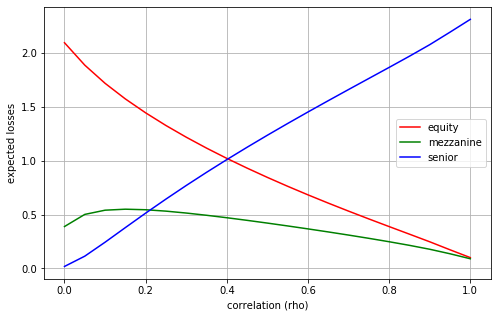
\includegraphics[width=0.7\linewidth]{figures/losses_vs_rho_2}
\end{center}
\end{figure}
To demonstrate that the total expected loss is independent from $\rho$ it is enough to print its values for a couple of different values of the correlation parameter. Since the expected loss of the tranches have been saved into lists the sum can be done among values of the lists with similar indices. 

\begin{ipython}
print (res[0][5] + res[1][5] + res[2][5])
print (res[0][10] + res[1][10] + res[2][10])
print (res[0][15] + res[1][15] + res[2][15])

2.4999999999999725
2.499999999999975
2.4999999999999774
\end{ipython}

\begin{question}
Using the \texttt{CollDebtObligation} class in the \texttt{finmarkets} module determine the fair value of each tranche in a CDO with 1 year maturity and a reference portfolio of 125 names. Each of them have the same default probabilities, 1\% and the correlation is set to 0.2. The tenor of the premium leg is 12 months. The risk free rate is flat at 5\%.
\begin{itemize}
	\item equity: [0.0, 0.03] (spread 0.20);
	\item mezzanine: [0.03, 0.06] (spread 0.01);
	\item senior: [0.06, 1.0] (spread 0.005).
\end{itemize}
How does these results change if the default probability raises to 5\% ? \\
How does these results change if instead there is an higher correlation (0.6) ?
\end{question}

\begin{solution}
\end{solution}

\begin{ipython}
from finmarkets import DiscountCurve, CreditCurve, CollDebtObligation
from datetime import date
from dateutil.relativedelta import relativedelta

pillar_dates = []
df = []
observation_date = date.today()

for i in range(2):
    pillar_dates.append(observation_date + relativedelta(years=i))
    df.append(1 / (1 + 0.05) ** i)
    dc = DiscountCurve(observation_date, pillar_dates, df)
cc = CreditCurve([observation_date + relativedelta(years=i) for i in range(5)],
    [1, 0.99, 0.97, 0.95, 0.93])
tranches = [[0.0, 0.03], [0.03, 0.06], [0.06, 0.09], [0.09, 1.0]]
spreads = [0.15, 0.07, 0.03, 0.01]
cdo = CollDebtObligation(100e6, 125, tranches, 0.3, cc,
    observation_date, spreads, 1, 12)
for i in range(len(tranches)):
    print ("Tranche {} ({}): {:.5f}".format(i, tranches[i], cdo.fair_value(i, dc)))

Tranche 0 ([0.0, 0.03]): 0.17775
Tranche 1 ([0.03, 0.06]): 0.01570
Tranche 2 ([0.06, 1.0]): 0.00012
\end{ipython}
With an higher default probability instead, the NPV of the default leg increases and so does the fair value.

\begin{ipython}
Tranche 0 ([0.0, 0.03]): 0.59296
Tranche 1 ([0.03, 0.06]): 0.22714
Tranche 2 ([0.06, 1.0]): 0.00530
\end{ipython}
Finally with a larger correlation the probability of multiple defaults increases leading to larger losses in safer tranches. So the fair value increases in mezzanine and senior tranches, but is lower in the equity where the probability of few defaults is reduced.

\begin{ipython}
Tranche 0 ([0.0, 0.03]): 0.09899
Tranche 1 ([0.03, 0.06]): 0.03498
Tranche 2 ([0.06, 1.0]): 0.00192
\end{ipython}
